\documentclass[12pt]{article}
\usepackage[utf8]{inputenc}
\usepackage[margin=1in,bottom=1.5in,a4paper]{geometry}
\usepackage{tikz}
\usepackage{amsmath}
\usepackage{amssymb}
\usepackage{multicol}
\usepackage{xcolor}
\usepackage{tabularx}
\usepackage{mathtools}
\usepackage{ textcomp }
\usepackage{graphicx}
\usepackage{ stmaryrd }
\usepackage{hyperref}
\usepackage{ marvosym }
\usepackage{ dsfont }
\usepackage{ulem}
\tolerance=1000
\usepackage{fancyhdr}
\pagestyle{fancy}
\headheight 50pt

\renewcommand{\thesection}{\Alph{section}}

%edit header and footer
\fancypagestyle{firstpage}{
  \lhead{*-as-a-Service cloud assets}
  \chead{\textbf{\Large Learnings}}
  \rhead{CySec Project '21}
}
\lhead{}
\rhead{*-as-a-Service cloud assets}

\cfoot{}
\rfoot{\small\thepage}

\begin{document}
\thispagestyle{firstpage}

\section*{Cloud Services}
\begin{itemize}
    \item \textbf{IaaS: Infrastructure as a Service} \\
    Users manage applications, data, operating system, middleware and runtimes. \\
    Provider is responsible for providing virtualization, storage, network and servers. \\
    \textit{Examples: AWS EC2, Rackspace, Google Compute Engine (GCE), Digital Ocean, Magento 1 Enterprise Edition, also Azure}
    
    \item \textbf{PaaS: Platform as a Service} \\
    Often used by: developers and programmers who have ideas for an app and can also program them, but do not have the infrastructure to operate and maintain it. \\
    \textit{Examples: AWS Elastic Beanstalk, Heroku, Microsoft Azure (mostly used as PaaS), Force.com, OpenShift, Apache Stratos, Magento Commerce Cloud}
    
    \item \textbf{SaaS: Software as a Service} \\
    Users interact with the software via a web browser. \\
    \textit{Examples: BigCommerce, Google Apps, Salesforce, Dropbox, MailChimp, ZenDesk, DocuSign, Slack, Hubspot, Paychex HR-Software, CA Technology Enterprise software, WordPress Content Management Software, Microsoft Office 365}
\end{itemize}

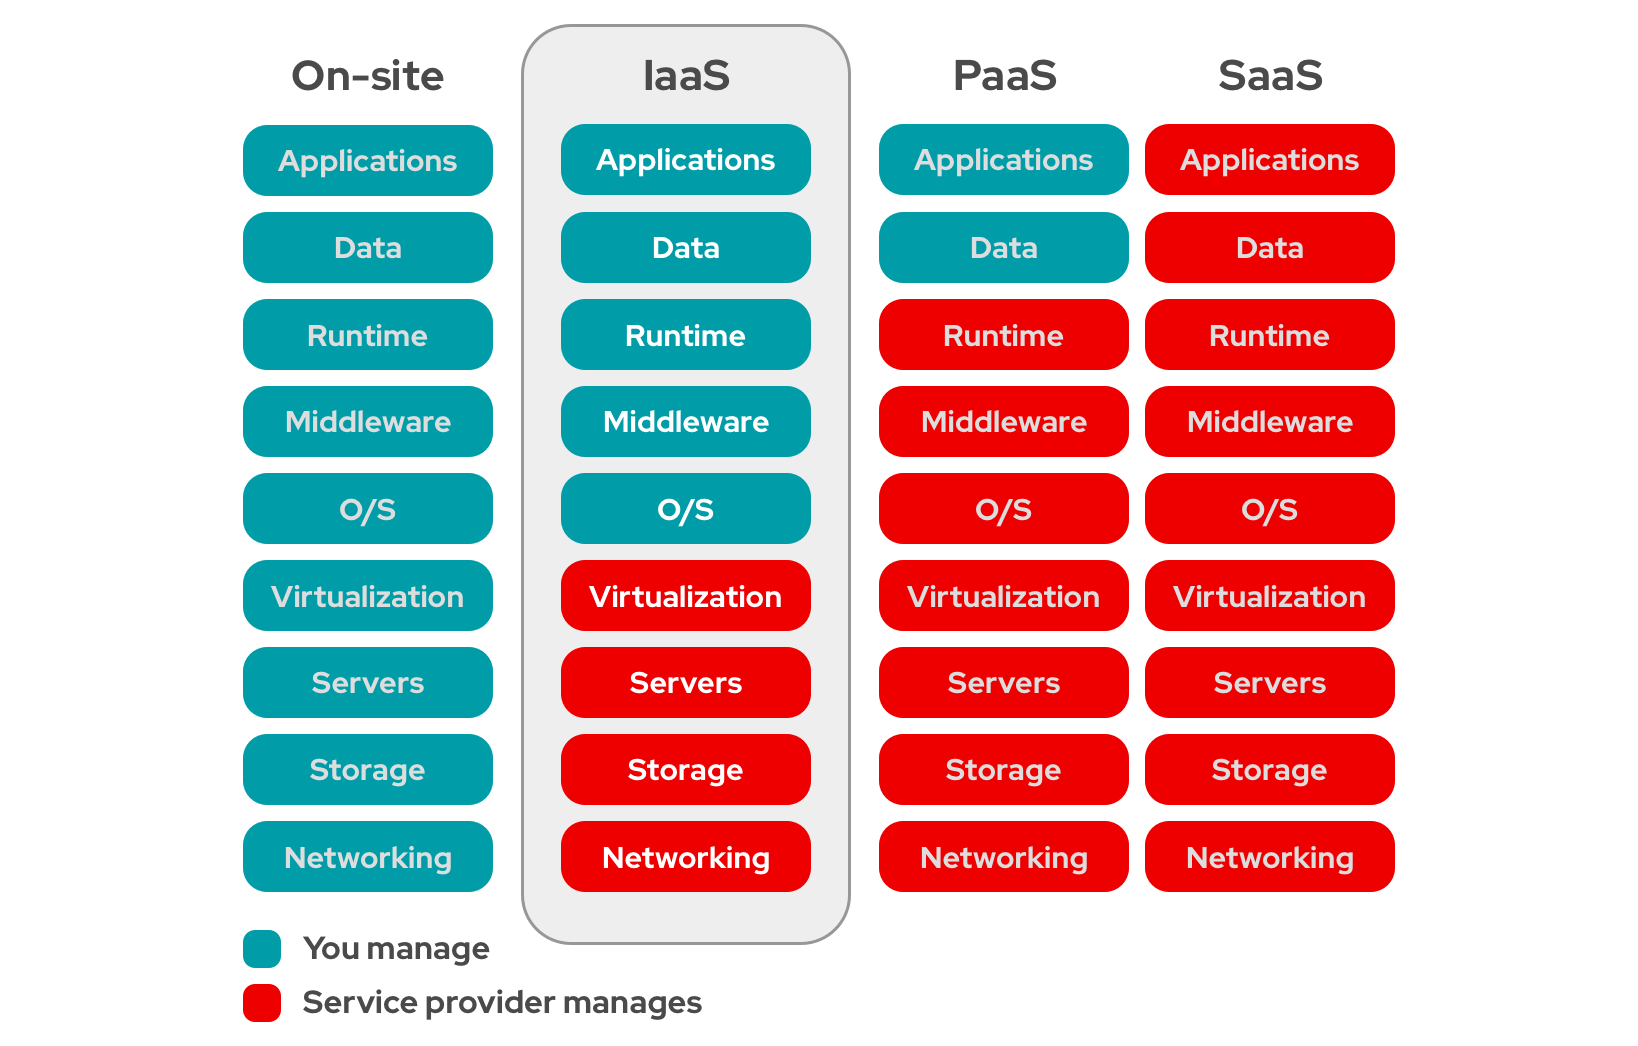
\includegraphics[scale=0.3]{as-a-Service_comparison.png}

\begin{center}
    \url{www.redhat.com/de/topics/cloud-computing/what-is-iaas}
\end{center}
"Most businesses use a combination of SaaS and IaaS cloud computing service models."

\section*{Cloud Providers} 
\textbf{Biggest Players} \hspace{11cm} \href{https://www.zdnet.com/article/the-top-cloud-providers-of-2021-aws-microsoft-azure-google-cloud-hybrid-saas/}{\textit{Source}}
\begin{enumerate}
    \item Amazon Web Services (AWS)
    \item Microsoft Azure
    \item Google Cloud and Anthos
    \item Alibaba Cloud (mainly China)
    \item IBM Cloud
    \item VMware (Dell)
\end{enumerate}
\textbf{Further Cloud Providers:}
\begin{itemize}
    \item Salesforce (leading in SaaS)
    \item Oracle Cloud
    \item SAP Business Technology Platform (SAP BTP)
    \item ServiceNow
    \item Microsoft Office 365
    \item OpenStack
    \item Kamatera
\end{itemize}

\section*{How to identify used Cloud Services}
\textbf{ToDo}

\newpage
\section*{Misc}
\begin{itemize}
    \item 
\end{itemize}
Everything that could be interesting in the future... 
\begin{itemize}
    \item ... to potentially identify which cloud service is used:
    \begin{itemize}
    \item Google Cloud offers \href{https://cloud.google.com/interconnect/docs/concepts/dedicated-overview}{\textit{Dedicated Interconnect}}
    \item AWS offers \href{https://aws.amazon.com/directconnect/}{\textit{Direct Connect}}
    \item Azure offers \href{https://azure.microsoft.com/en-us/services/expressroute/}{\textit{ExpressRoute}}
    \item OpenStack offers \href{https://www.openstack.org/passport/}{\textit{OpenStack Public Cloud Passport}}
\end{itemize}
\end{itemize}

\end{document}
